\hypertarget{product_8inc}{
\section{include/product.inc File Reference}
\label{product_8inc}\index{include/product.inc@{include/product.inc}}
}
Functions to output Product Info. 

\subsection*{Functions}
\begin{CompactItemize}
\item 
\hyperlink{product_8inc_9dbb778854cfe105058d7161ca8f058c}{getImages} (\$product)
\end{CompactItemize}


\subsection{Detailed Description}
Functions to output Product Info. 

Various pieces of info gleamed from the web will be handled by functions contained in this file. Currently, it only handles getting product images 

Definition in file \hyperlink{product_8inc-source}{product.inc}.

\subsection{Function Documentation}
\hypertarget{product_8inc_9dbb778854cfe105058d7161ca8f058c}{
\index{product.inc@{product.inc}!getImages@{getImages}}
\index{getImages@{getImages}!product.inc@{product.inc}}
\subsubsection{\setlength{\rightskip}{0pt plus 5cm}getImages (\$ {\em product})}}
\label{product_8inc_9dbb778854cfe105058d7161ca8f058c}


Gets Appropriate Images from google Image Search \begin{Desc}
\item[Parameters:]
\begin{description}
\item[{\em \$product}]The product to get images for \end{description}
\end{Desc}
\begin{Desc}
\item[Returns:]HTML code to output product images \end{Desc}


Definition at line 15 of file product.inc.

References fget().

Referenced by getBarcodeInfo().

\begin{Code}\begin{verbatim}15                              {
19   $json = json_decode(fget('http://ajax.googleapis.com/ajax/services/search/images?v=1.0&q=' . urlencode($product) . '&rsz=large'));
20   // Hack to get Indexes working
21   if ($_GET['index']) {
22     $currentIndex = (int) $_GET['index'];
23   }
24   else {
25     $currentIndex = 0;
26   }
27   $prevIndex = $currentIndex - 1;
28   $nextIndex = $currentIndex + 1;
29   $i = 0;
30   $getText = '?';
31   foreach ($_GET as $item) {
32     if (key($_GET) != 'index') {
33       if ($i == 0) {
34         $getText .= key($_GET) . '=' . $item;
35       }
36       else {
37         $getText .= '&' . key($_GET) . '=' . $item;
38       }
39     }
40     next($_GET);
41     $i++;
42   }
43 
44   $originalContextUrl = $json->responseData->results[$currentIndex]->originalContextUrl;
45   $imgSrc = $json->responseData->results[$currentIndex]->tbUrl;
46   $visibleUrl = $json->responseData->results[$currentIndex]->visibleUrl;
47 
51   $output = "<div id=\"prodimg\">";
52   // Only display previous button if there are previous values
53   if ($currentIndex > 0) {
54     $output .= "<a href=\"{$getText}&index={$prevIndex}\"><img src=\"images/arrows/left.png\" alt=\"Previous Image\" title=\"Previous Image\" /></a>";
55   }
56   $output .= "<a href=\"{$originalContextUrl}\" target=\"_blank\"><img src=\"{$imgSrc}\" alt=\"Image of $product From {$visibleUrl}\" title=\"Image of $product From {$visibleUrl}\" id=\"prodimg\"></a>";
57   // Only display next button if there are more images
58   if ($currentIndex < count($json->responseData->results) - 1) {
59    $output .= "<a href=\"{$getText}&index={$nextIndex}\"> <img src=\"images/arrows/right.png\" alt=\"Next Image\" title=\"Next Image\" /></a><br /><a href=\"aboutimages.html\" target=\"_blank\" onclick=\"popup(this.href, 200, 300); return false;\">About this image</a></div>";
60   }
61 
62   return $output;
63 }
\end{verbatim}
\end{Code}




Here is the call graph for this function:\nopagebreak
\begin{figure}[H]
\begin{center}
\leavevmode
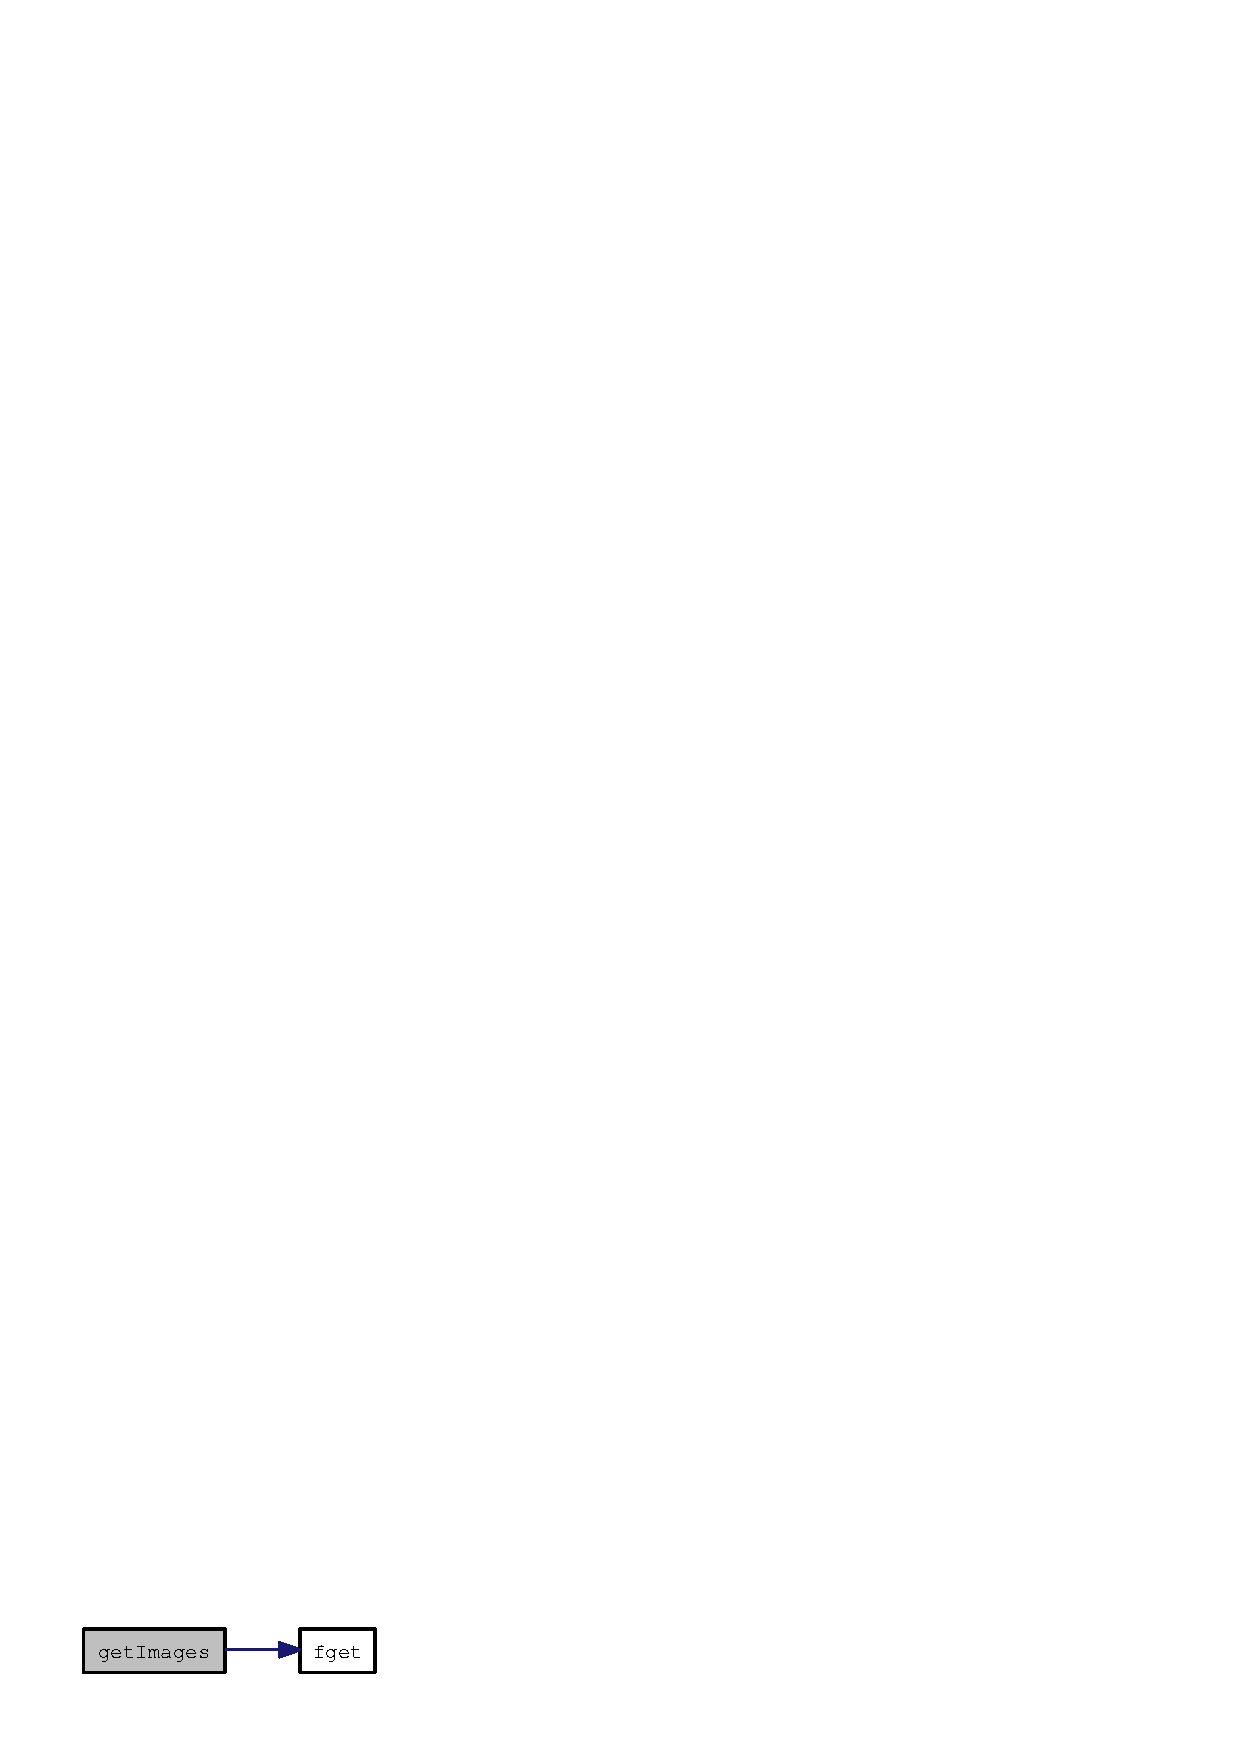
\includegraphics[width=92pt]{product_8inc_9dbb778854cfe105058d7161ca8f058c_cgraph}
\end{center}
\end{figure}


Here is the caller graph for this function:\nopagebreak
\begin{figure}[H]
\begin{center}
\leavevmode
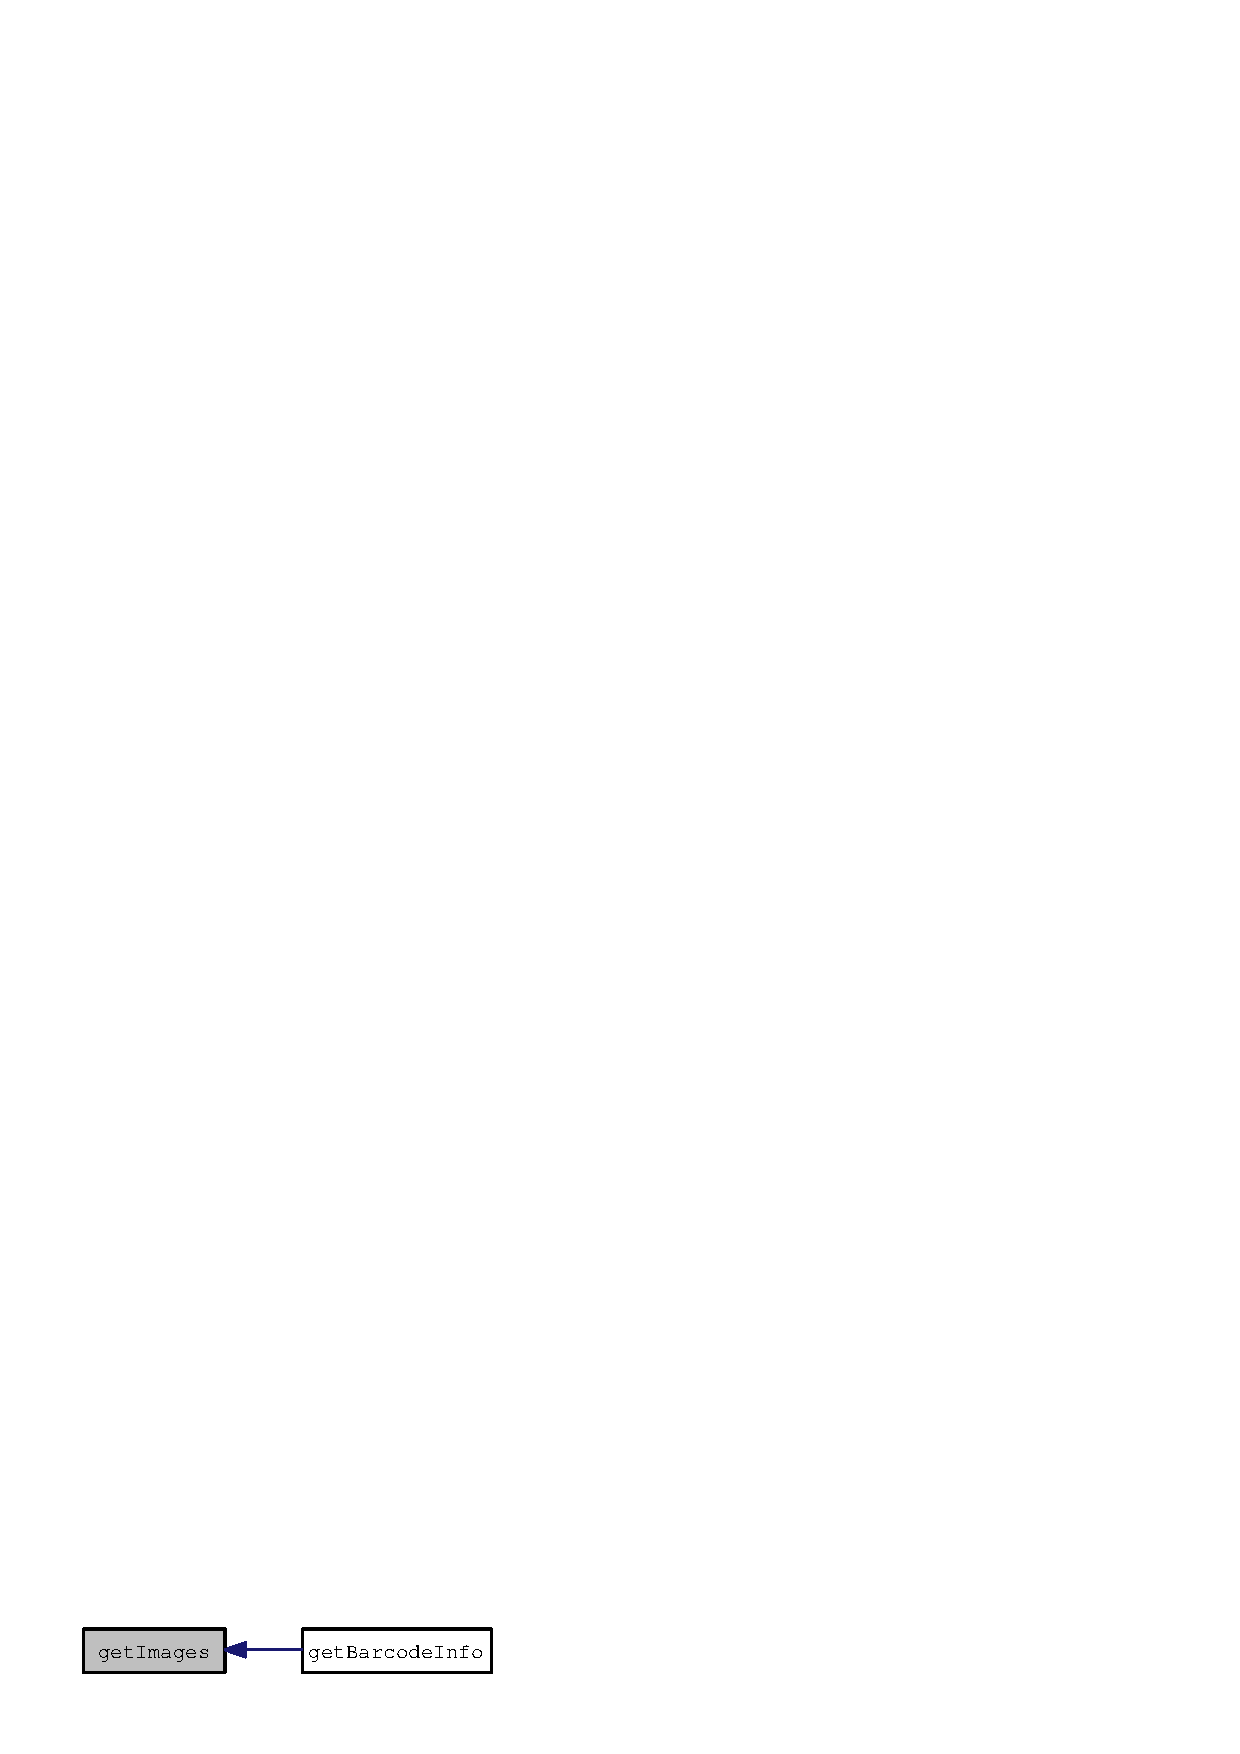
\includegraphics[width=120pt]{product_8inc_9dbb778854cfe105058d7161ca8f058c_icgraph}
\end{center}
\end{figure}
